\documentclass[twocolumn,10pt]{ltjsarticle}

\usepackage[top=20mm,bottom=20mm,left=25mm,right=25mm,columnsep=10mm]{geometry}
\usepackage[haranoaji,nfssonly]{luatexja-preset}
\usepackage{graphicx}
\usepackage{titlesec}
\usepackage{url}

\titleformat*{\section}{\Large\bfseries}
\titleformat*{\subsection}{\large\bfseries}

\title{【実験】LombScargleピリオドグラムによるShinoBot通信の解析}
\author{山下 尚彦}
\date{\today}

\begin{document}
\maketitle

\section{はじめに}
私の卒業研究ではボットとなったPCを特定するために, ボットとC2サーバ間の通信を解析する手法を提案した. 
C2サーバとは攻撃者がボットネットを操作するための用意したサーバのことで, C2サーバを介して攻撃命令などを行う. 
また, C2サーバはボットネットが運用可能かどうかを確認するために定期的に通信を行う. 
私の提案手法ではネットワーク上の通信を収集し, 周期性のある通信を検出することでボットの検出を行った. 
しかし, 卒業研究の段階では周期性があるかを判断するには画像を見る必要があったため, 
ネットワーク上に多数の端末があった場合, そのすべての通信の画像を見る作業は困難であり, 実用的ではなかった. 

\section{概要}
\subsection{周期性のある通信の検出手法}
提案手法では, 通信の周期性を推定するためにLomb-Scargleピリオドグラム\cite{vanderplas2018understanding}を用いた. 
このピリオドグラムは不定間隔, または欠損のある信号であっても周波数解析を行えるため, 
\textbf{図\ref{fig:lombscargle}}のような連続していない正弦波の周期性を推定することができる. 

\begin{figure}[htb]
    \centering
    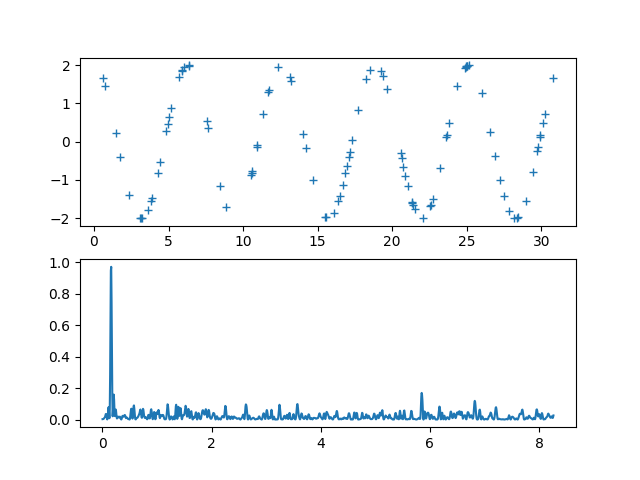
\includegraphics[width=8cm]{images/【実験】LombScargleピリオドグラムによるShinoBot通信の解析/lombscargle.png}
    \caption{欠損のある正弦波と解析結果}
    \label{fig:lombscargle}
\end{figure}

\subsection{周期性の測定方法}
Lomb-Scargleピリオドグラムによる信号の周期性はピークを用いることで判断することができる. 
これは, 信号が周期性のない正規分布だという過程に基づいてある一定の値以上のピークを解析結果が示した場合によって判断される. 
図\ref{fig:lombscargle}を例にすると, 図の正弦波が非周期的である確率が0.1\%以上, 
つまり99.9\%周期的であるためには, 図のグラフのピークが0.18631798(${=P_{0.1}}$)以上であることを意味する. 
このグラフのピークは0.9993959064009751と, ${P_{0.1}}$を超えているため99.9\%以上周期的であると言える. 

\section{実験}
卒業研究では, ボットやリモートアクセルツールのシミュレーションが行えるShinoBotを, 
仮想マシン上のWindows10で実行して実験を行った. 
また, LINEやSlackなどのコミュニケーションツールやウェブブラウジングをしてShinoBot以外の通信を発生させた. 

\section{結果}
実験の結果, ShinoBotとC2サーバ間の周期的な通信を検出できた. 
図\ref{fig:shinobot}の上のグラフはShinoBotとC2サーバの通信回数と通信時間の関係をグラフにしたもので, 
Lomb-Scargleピリオドグラムで解析した結果が下のグラフである. 
図\ref{fig:shinobot}の上のグラフの横軸は00時00分00秒から23時59分59秒までの経過秒数を表し, 
縦軸は通信回数を表す. 図\ref{fig:shinobot}からC2サーバとの通信回数は10秒ごとに1, 2回, 
まれに3回以上通信を行っていることがわかる. 
下のグラフの横軸は周波数を表し, 縦軸はパワースペクトル密度を表している. 
ピークが0.5857179088094826で, 99.9\%周期的であるには0.00289756以上である必要があるが, 
この値をピークが超えているため周期性があると考えられる. 
このグラフから, 0.10Hzにピークが現れているため, 通信の周期は周波数0.10Hzの逆数の10秒であるとわかる. 
これはShinoBotとC2サーバ間の通信間隔と一致しているため実験の結果は正しいと言える. 

\begin{figure}[htb]
    \centering
    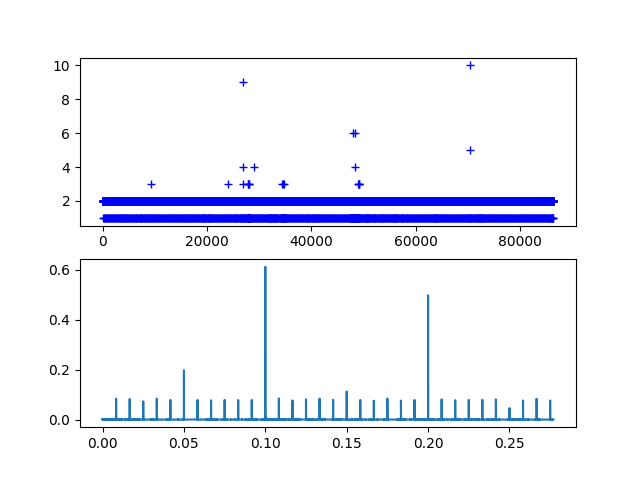
\includegraphics[width=8cm]{images/【実験】LombScargleピリオドグラムによるShinoBot通信の解析/shinobot.png}
    \caption{C2サーバとの通信回数と解析結果}
    \label{fig:shinobot}
\end{figure}

\section{考察}
今回の実験で, 周期性のある通信を画像を頼らずに絞り込むことができるとわかった. 
しかし, 99.9\%周期的である通信で絞り込むと10000の通信中2000と依然数が多かった. 
これは他のアプリケーションで周期的な通信を行っていたものや通信回数が少なかったり, 
極端に多かった通信が含まれていたことに原因があると考えられる. 
今後は, 確率の値をどの程度変更することできるかや他のデータセットを用いて, 実験を行いたいと思う. 

\section{おわりに}
本実験メモでは, Lomb-Scargleピリオドグラムの概要と周期性の測定方法と卒業研究での実験を基に
機械的に周期性のある通信の絞り込みを行う実験を行った. 
その結果, ある程度絞り込むことができたが依然画像をみて周期性の判別を行うには困難な量の通信を検出したため, 
今後は, 値を変えたり他のデータセットを用いて検証し, 問題の解決を検討したいと思う. 

\bibliographystyle{junsrt}
\bibliography{DB}
\end{document}